% Golden Spiral can be approximated with Golden ratio or Fibonacci sequence.
% Golden Ratio: a+b/a = a/b

\documentclass{beamer}
\usepackage[utf8]{inputenc}
\usepackage[T1]{fontenc}

\usepackage{hyperref}
\hypersetup{
    colorlinks=true,
    linkcolor=blue,
    filecolor=magenta,      
    urlcolor=cyan,
}

\usetheme{Cuerna}
\usecolortheme{default}
% default, bluesimplex, lettuce, brick

% slide (frames) numbering
\addtobeamertemplate{navigation symbols}{}{
    \usebeamerfont{footline}%
    \usebeamercolor[fg]{footline}%
    \hspace{1em}%
    \insertframenumber/\inserttotalframenumber
}

\title{Gradient Descent Algorithms}
\author{Shayan Amani}

\date{spring '19}
\institute{Department of Computer Science, University of New Hampshire}

\begin{document}

  \begin{frame}
    \titlepage
  \end{frame}

\begin{frame}
    \frametitle{Introduction}
    % \framesubtitle{SUB}
    
    There are numerous varients of GD algorithms:
    \begin{itemize}
        \item Batch gradient descent
        \item
    \end{itemize}
    
   
    Adam optimizer's paper: https://arxiv.org/pdf/1412.6980.pdf

  \end{frame}
  
\begin{frame}
    \frametitle{Motivation}
    Almost every prominent differentiable programming frameworks are using Gradient Descent-based optimizers. 
    
    \begin{table}[]
        \centering
        \begin{tabular}{c|c}
                
\includegraphics[scale=0.1]{tf-logo-vertical.png}
 &      
\includegraphics[scale=0.15]{pytorch-logo-vertical.png}
\\
\hline
            
\includegraphics[scale=0.15]{caffe-logo.png}
     &     
\includegraphics[scale=0.2]{cntk-logo.png}
\\
        \end{tabular}
        \label{tab:logos-motivation}
    \end{table}
    
\end{frame}
  
\begin{frame}
    \frametitle{Motivation}
    \framesubtitle{TensorFlow}
    
    \begin{table}
        \centering
        \begin{tabular}{c}
        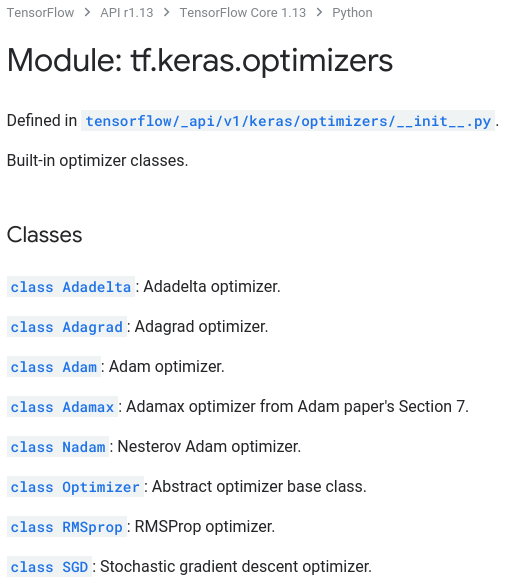
\includegraphics[scale=0.3]{tf-keras-optimizers.png}
 \\
        \end{tabular}
        \label{tab:tf-motivation}
    \end{table}
    
\end{frame}

\begin{frame}
    \frametitle{Motivation}
    \framesubtitle{PyTorch}
    
    \begin{table}
        \centering
        \begin{tabular}{c c}
        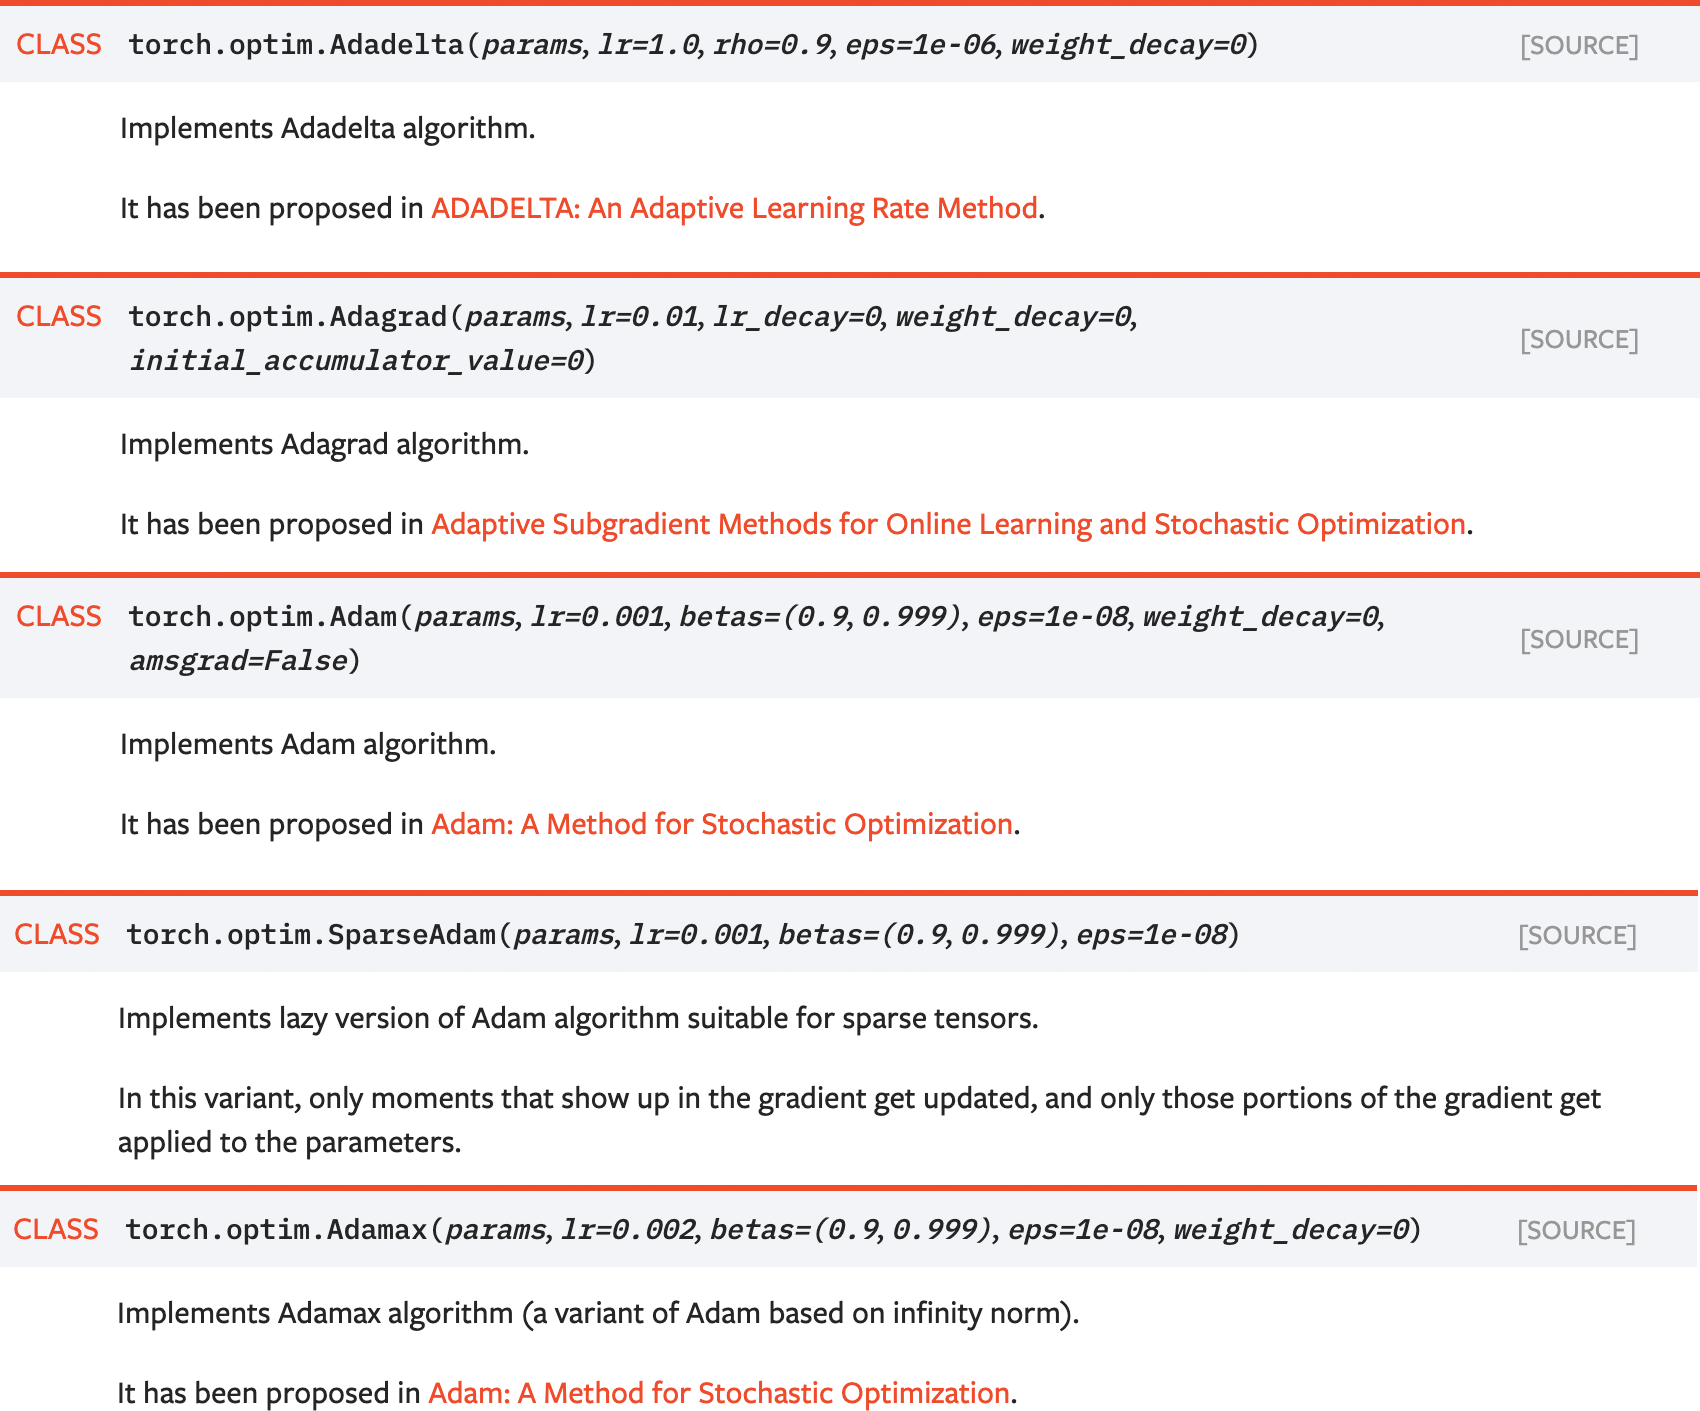
\includegraphics[width=0.5\columnwidth]{pytorch-algs-1.png} & 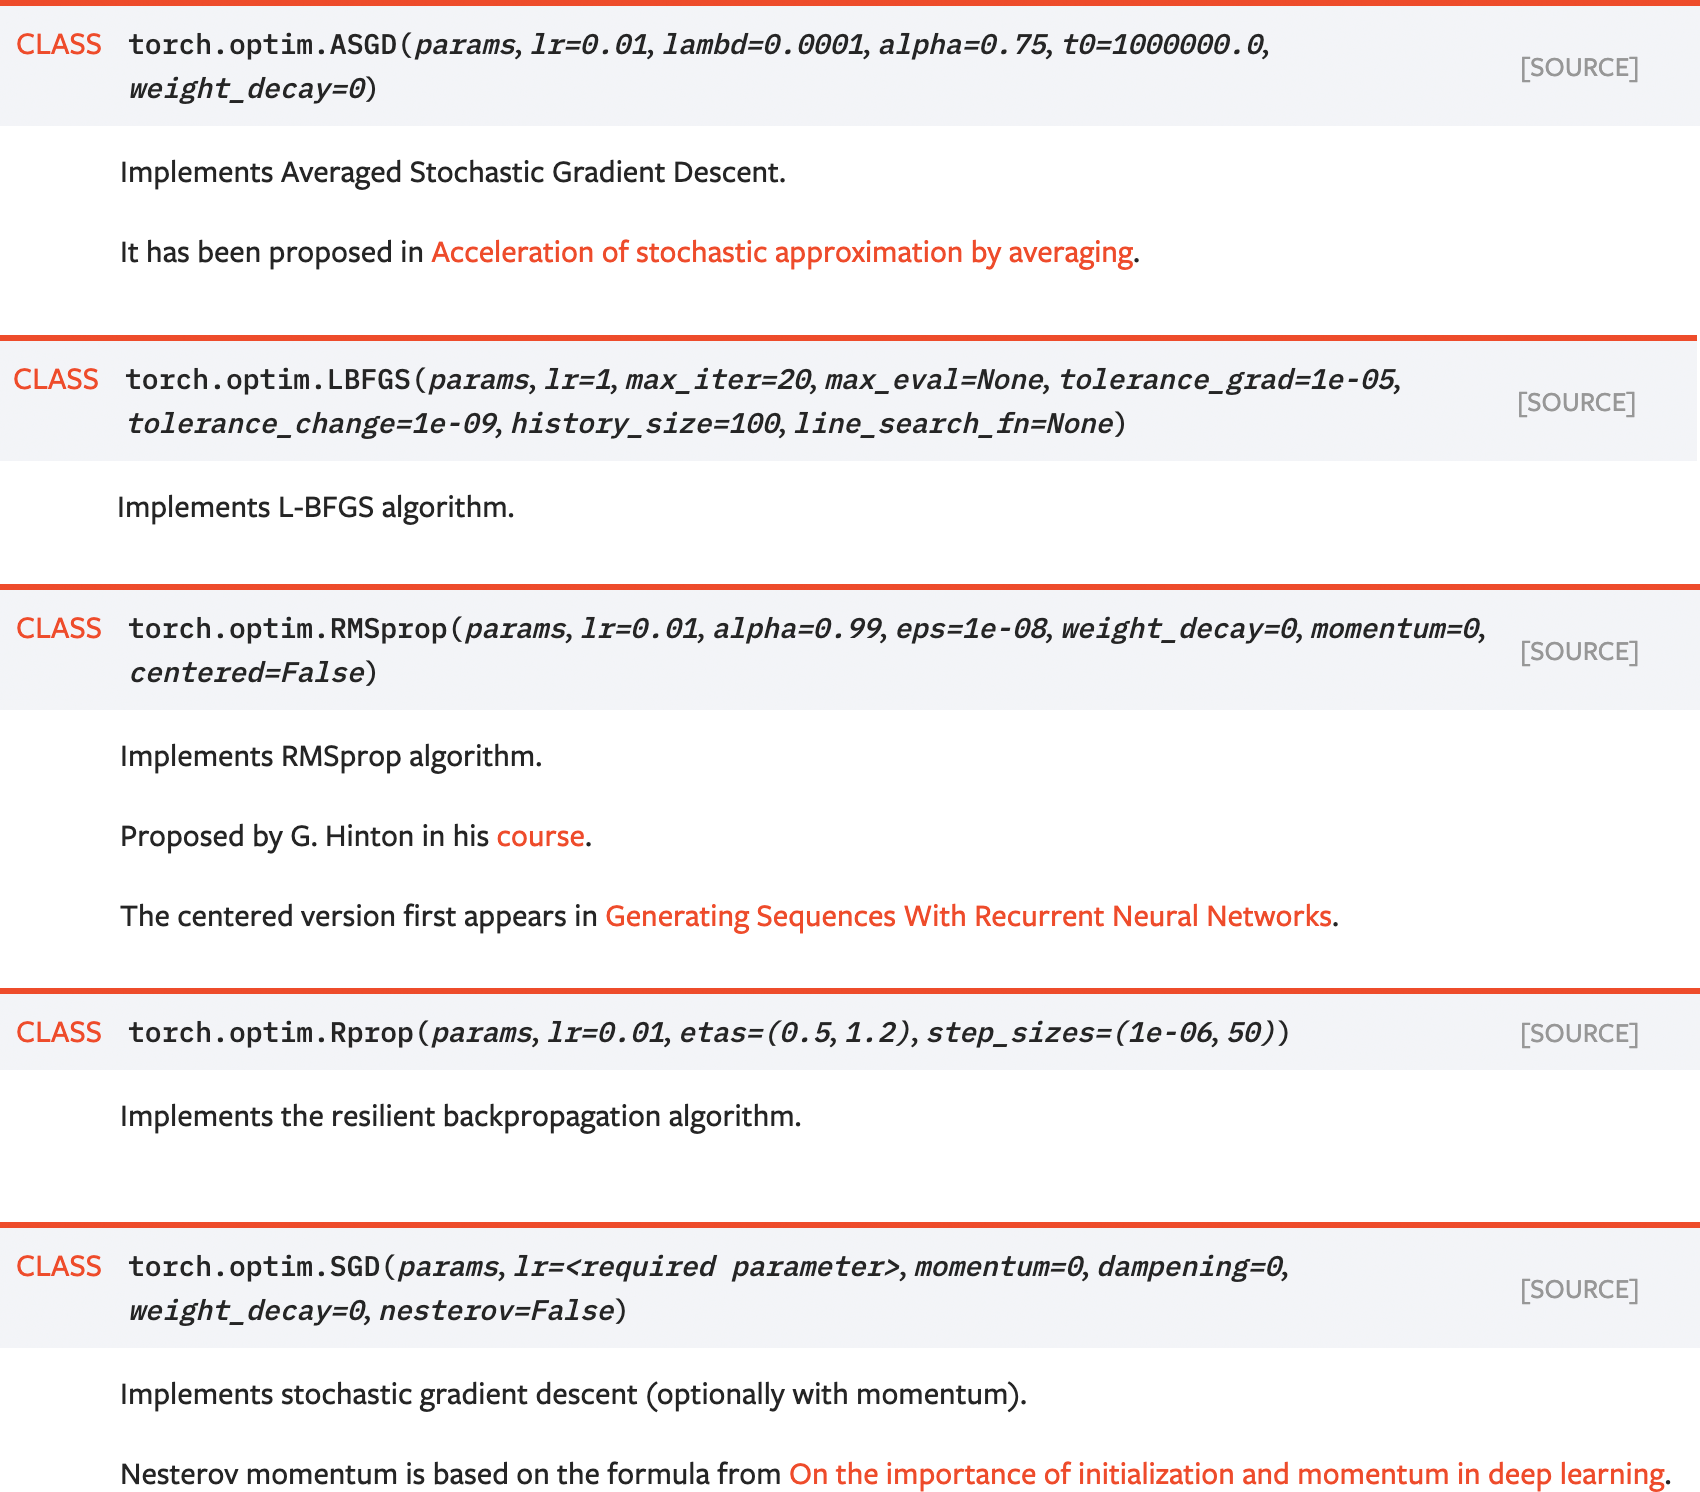
\includegraphics[width=0.5\columnwidth]{pytorch-algs-2.png} 
 \\
        \end{tabular}
        \label{tab:pytorch-motivation}
    \end{table}
    
\end{frame}

\begin{frame}
    \frametitle{Motivation}
    \framesubtitle{Caffe}
    
    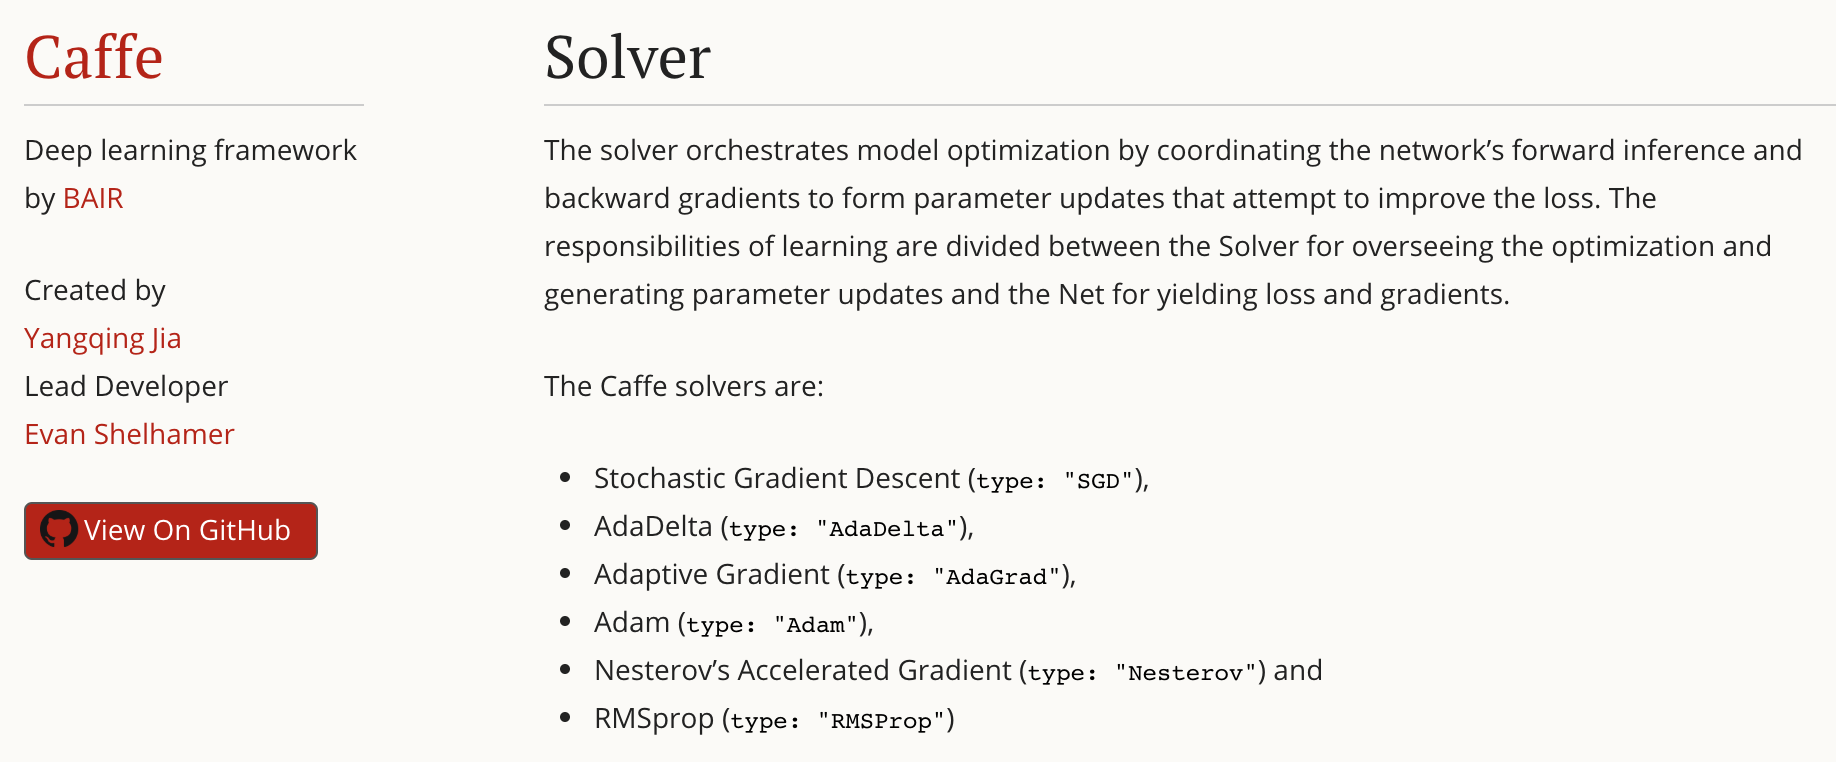
\includegraphics[width=1\columnwidth]{caffe-algs.png}
    
\end{frame}

\begin{frame}
    \frametitle{Motivation}
    \framesubtitle{Microsoft Cognitive Toolkit}
    
    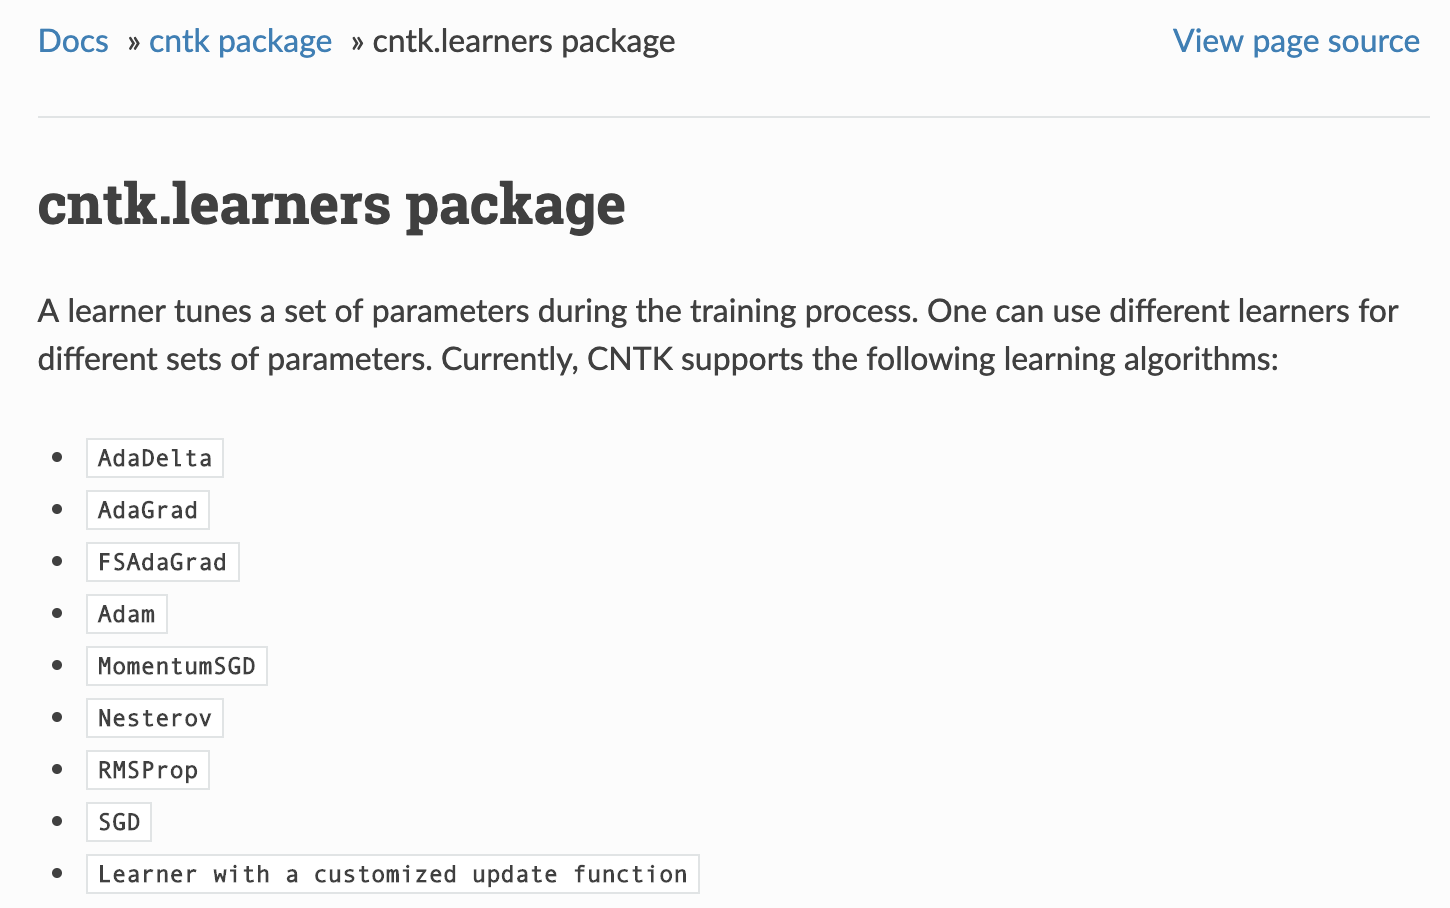
\includegraphics[width=1\columnwidth]{cntk-algs.png}
    
\end{frame}
\end{document}
